\documentclass[11pt,a4paper]{article}
\usepackage[margin=2.2cm]{geometry}
\usepackage{lmodern}
\usepackage[T1]{fontenc}
\usepackage{xcolor}
\usepackage{tikz}
\usetikzlibrary{arrows.meta,positioning,fit,calc}
\usepackage{booktabs}
\usepackage{eurosym}
\usepackage{enumitem}
\usepackage[hidelinks]{hyperref}

% site palette
\definecolor{navy}{HTML}{1C1C2E}
\definecolor{surface}{HTML}{25253A}
\definecolor{accent}{HTML}{3BA8C0}
\definecolor{mgreen}{HTML}{5E9A45}
\definecolor{myellow}{HTML}{C77F2E}
\definecolor{mred}{HTML}{D94F42}
\definecolor{mpurple}{HTML}{7A5490}
\definecolor{mutedg}{HTML}{666680}

\tikzset{
  box/.style={draw=#1, thick, rounded corners=3pt, fill=#1!8, text=navy,
              align=center, minimum height=9mm, inner sep=2.5mm, font=\small},
  flow/.style={-{Stealth[length=3mm]}, thick, draw=#1},
  lbl/.style={font=\scriptsize, text=mutedg, align=center},
  step/.style={draw=#1, thick, rounded corners=2pt, fill=#1!10, text=navy,
               align=left, inner sep=2mm, font=\scriptsize}
}

\setlength{\parindent}{0pt}
\setlength{\parskip}{4pt}

\title{\vspace{-1.4cm}\textbf{lcecon.ie} $\times$ \textbf{CSO PxStat}\\
\large The live data pipeline, at a glance}
\author{}
\date{July 2026 --- every fact verified against the live API}

\begin{document}
\maketitle
\vspace{-1.2cm}

\section*{1\quad The whole system}

\begin{center}
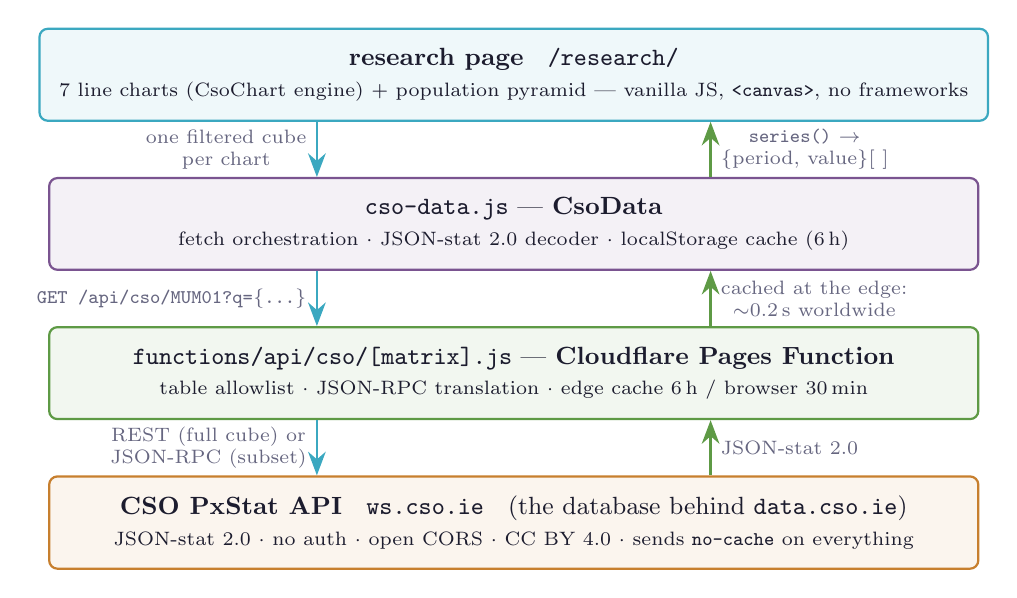
\begin{tikzpicture}[node distance=7mm]
  \node[box=accent, minimum width=118mm] (page)
    {\textbf{research page} \; \texttt{/research/}\\
     \scriptsize 7 line charts (CsoChart engine) + population pyramid --- vanilla JS, \texttt{<canvas>}, no frameworks};
  \node[box=mpurple, minimum width=118mm, below=of page] (data)
    {\texttt{cso-data.js} --- \textbf{CsoData}\\
     \scriptsize fetch orchestration \(\cdot\) JSON-stat 2.0 decoder \(\cdot\) localStorage cache (6\,h)};
  \node[box=mgreen, minimum width=118mm, below=of data] (proxy)
    {\texttt{functions/api/cso/[matrix].js} --- \textbf{Cloudflare Pages Function}\\
     \scriptsize table allowlist \(\cdot\) JSON-RPC translation \(\cdot\) edge cache 6\,h / browser 30\,min};
  \node[box=myellow, minimum width=118mm, below=of proxy] (cso)
    {\textbf{CSO PxStat API} \; \texttt{ws.cso.ie} \; (the database behind \texttt{data.cso.ie})\\
     \scriptsize JSON-stat 2.0 \(\cdot\) no auth \(\cdot\) open CORS \(\cdot\) CC BY 4.0 \(\cdot\) sends \texttt{no-cache} on everything};
  \draw[flow=accent]  ($(page.south)+(-25mm,0)$) -- ($(data.north)+(-25mm,0)$)
      node[midway,left,lbl]{one filtered cube\\per chart};
  \draw[flow=accent]  ($(data.south)+(-25mm,0)$) -- ($(proxy.north)+(-25mm,0)$)
      node[midway,left,lbl]{\texttt{GET /api/cso/MUM01?q=\{...\}}};
  \draw[flow=accent]  ($(proxy.south)+(-25mm,0)$) -- ($(cso.north)+(-25mm,0)$)
      node[midway,left,lbl]{REST (full cube) or\\JSON-RPC (subset)};
  \draw[flow=mgreen]  ($(cso.north)+(25mm,0)$) -- ($(proxy.south)+(25mm,0)$)
      node[midway,right,lbl]{JSON-stat 2.0};
  \draw[flow=mgreen]  ($(proxy.north)+(25mm,0)$) -- ($(data.south)+(25mm,0)$)
      node[midway,right,lbl]{cached at the edge:\\$\sim$0.2\,s worldwide};
  \draw[flow=mgreen]  ($(data.north)+(25mm,0)$) -- ($(page.south)+(25mm,0)$)
      node[midway,right,lbl]{\texttt{series()} $\to$\\\{period, value\}[ ]};
\end{tikzpicture}
\end{center}

Deploy is \emph{push to main}: Cloudflare Pages rebuilds the static site and the
proxy function together, $\sim$1 minute, zero configuration.

\section*{2\quad Why a proxy? The four-level fallback}

The CSO sends \texttt{cache-control: no-cache} on every response, so without our
own caching every student pays a cold round trip to CSO origin. The page also
never breaks: each level below catches the failure of the one above.

\begin{center}
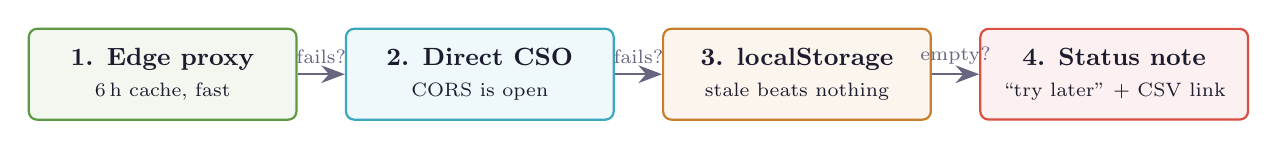
\begin{tikzpicture}[node distance=4mm and 6mm]
  \node[box=mgreen,  minimum width=34mm] (l1) {\textbf{1. Edge proxy}\\\scriptsize 6\,h cache, fast};
  \node[box=accent,  minimum width=34mm, right=of l1] (l2) {\textbf{2. Direct CSO}\\\scriptsize CORS is open};
  \node[box=myellow, minimum width=34mm, right=of l2] (l3) {\textbf{3. localStorage}\\\scriptsize stale beats nothing};
  \node[box=mred,    minimum width=34mm, right=of l3] (l4) {\textbf{4. Status note}\\\scriptsize ``try later'' + CSV link};
  \draw[flow=mutedg] (l1) -- (l2) node[midway,above,lbl]{fails?};
  \draw[flow=mutedg] (l2) -- (l3) node[midway,above,lbl]{fails?};
  \draw[flow=mutedg] (l3) -- (l4) node[midway,above,lbl]{empty?};
\end{tikzpicture}
\end{center}

Level 2 also covers local development (\texttt{python3 -m http.server} runs no
Pages Functions), so the same code works everywhere unchanged.

\section*{3\quad Decoding JSON-stat: the one piece of real arithmetic}

A cube arrives as one flat \texttt{value[]} array plus its dimensions. The flat
index is row-major over the \texttt{id} order --- exactly like nested loops:

\begin{center}
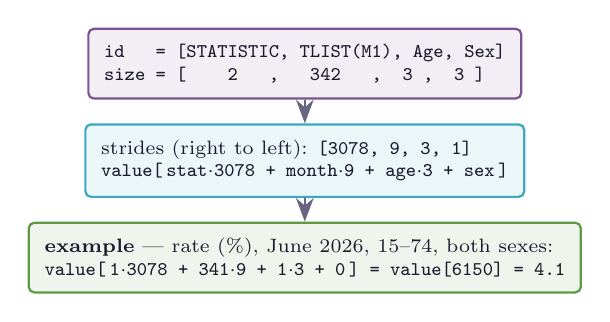
\begin{tikzpicture}[node distance=3mm and 8mm]
  \node[step=mpurple] (meta) {%
    \texttt{id\ \ \ = [STATISTIC,\ TLIST(M1),\ Age,\ Sex]}\\
    \texttt{size = [\ \ \ \ 2\ \ \ ,\ \ \ 342\ \ \ ,\ \ 3\ ,\ \ 3\ ]}};
  \node[step=accent, below=of meta] (stride) {%
    strides (right to left): \texttt{[3078,\ 9,\ 3,\ 1]}\\
    \texttt{value[\,stat$\cdot$3078 + month$\cdot$9 + age$\cdot$3 + sex\,]}};
  \node[step=mgreen, below=of stride] (ex) {%
    \textbf{example} --- rate (\%), June 2026, 15--74, both sexes:\\
    \texttt{value[\,1$\cdot$3078 + 341$\cdot$9 + 1$\cdot$3 + 0\,] = value[6150] = 4.1}};
  \draw[flow=mutedg] (meta) -- (stride);
  \draw[flow=mutedg] (stride) -- (ex);
\end{tikzpicture}
\end{center}

\texttt{CsoData.series(ds, fixed)} does this for a whole time axis: pin every
non-time dimension, walk the time categories, return
\texttt{[\{code, label, value\}]}. One PxStat quirk: \texttt{category.index} is
an \emph{array} of codes (Eurostat uses an object) --- the decoder handles both.

\section*{4\quad Anatomy of a chart block}

\begin{center}
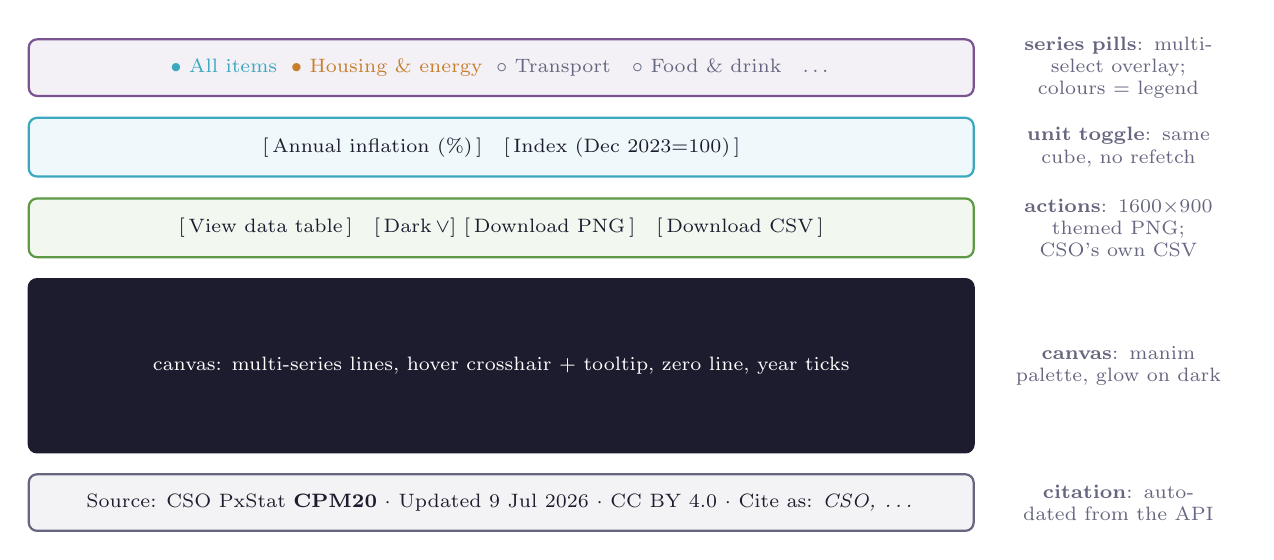
\begin{tikzpicture}[node distance=2.5mm]
  \node[box=mpurple, minimum width=120mm, minimum height=7mm] (pills)
    {\scriptsize \textcolor{accent}{$\bullet$ All items}\;
     \textcolor{myellow}{$\bullet$ Housing \& energy}\;
     \textcolor{mutedg}{$\circ$ Transport \; $\circ$ Food \& drink \; \dots}};
  \node[lbl, right=2mm of pills, text width=30mm] {\textbf{series pills}: multi-select overlay; colours = legend};
  \node[box=accent, minimum width=120mm, minimum height=6mm, below=of pills] (stats)
    {\scriptsize [\,Annual inflation (\%)\,] \; [\,Index (Dec 2023=100)\,]};
  \node[lbl, right=2mm of stats, text width=30mm] {\textbf{unit toggle}: same cube, no refetch};
  \node[box=mgreen, minimum width=120mm, minimum height=6mm, below=of stats] (act)
    {\scriptsize [\,View data table\,] \; [\,Dark\,$\vee$] [\,Download PNG\,] \; [\,Download CSV\,]};
  \node[lbl, right=2mm of act, text width=30mm] {\textbf{actions}: 1600$\times$900 themed PNG; CSO's own CSV};
  \node[box=navy, minimum width=120mm, minimum height=22mm, below=of act, fill=navy] (canvas)
    {\textcolor{white}{\scriptsize canvas: multi-series lines, hover crosshair
     + tooltip, zero line, year ticks}};
  \node[lbl, right=2mm of canvas, text width=30mm] {\textbf{canvas}: manim palette, glow on dark};
  \node[box=mutedg, minimum width=120mm, minimum height=7mm, below=of canvas] (cap)
    {\scriptsize Source: CSO PxStat \textbf{CPM20} \(\cdot\) Updated 9 Jul 2026 \(\cdot\)
     CC BY 4.0 \(\cdot\) Cite as: \emph{CSO, \dots}};
  \node[lbl, right=2mm of cap, text width=30mm] {\textbf{citation}: auto-dated from the API};
\end{tikzpicture}
\end{center}

The engine builds all of this from a $\sim$20-line config; the pill list comes
from live metadata, so new CSO categories appear automatically.

\section*{5\quad The visualisation suite and its tables}

Three renderers share one data layer: \textbf{lines} (CsoChart), \textbf{donuts}
with a year slider (CsoPie), and the \textbf{regional map} (CsoMap). A third
build round added twenty more visuals — BoP in depth (BPQ15), reserve assets
(BPQ18), UK trade and FDI after Brexit (BPQ35/38), energy dependence and demand
(SEI01/06, TSM10, MEC02), aircraft leasing (ALIA01/03/09) and the international
investment position and external debt (BPQ26/24) — with written analysis blocks
on the page. The donut engine gained \texttt{annualize} (quarterly/monthly
$\to$ annual sums) and \texttt{signed} (magnitude slices, sign in legend) for
balance-of-payments data. Full inventory: \texttt{cso-data-pipeline.md}. The
original charts:

\begin{center}\small
\begin{tabular}{@{}llll@{}}
\toprule
\textbf{Chart} & \textbf{Table} & \textbf{Span} & \textbf{Pills / toggle / slider}\\
\midrule
Unemployment          & MUM01 & 1998-- (monthly) & 3 ages / \% vs '000s\\
Inflation (CPI)       & CPM20 & 1996-- (monthly) & 14 commodity groups / \% vs index\\
GDP--GNP--GNI--GNI*   & NA001 & 1995-- (annual)  & 4 aggregates, \euro{}bn\\
House prices          & HPM09 & 2005-- (monthly) & 6 regions/types / index vs \%\\
Dwelling completions  & NDQ01 & 2011-- (quarterly) & 4 house types / raw vs SA\\
Government debt       & GFQ12 & 2000-- (quarterly) & single series, \% of GDP\\
Merchandise trade     & TSM01 & 1970-- (monthly) & exports, imports, surplus ($\pm$SA)\\
Population pyramid    & PEA11 & 1926-- (year slider) & single year of age $\times$ sex\\
\addlinespace
Tax revenue (donut)   & ITXS01 & 1995-- (year slider) & top-9 tax heads + Other\\
Gov.\ rev/exp/deficit & GFA01 & 1995-- (annual) & revenue, expenditure, B9\\
Social protection (donut) & SPEA02 & 2000-- (year slider) & 9 benefit functions\\
Balance of payments   & BPQ15 & 2002-- (quarterly) & current acct, goods, services, income\\
Trade in services     & BPA04 & 2003-- (annual) & 8 components / exports vs imports\\
Industrial production & MIM05 & 2015-- (monthly) & modern vs traditional sector\\
Retail sales          & RSM08 & 2021-- (monthly) & 6 business types / volume vs value\\
Services index        & MSI03 & 2021-- (monthly) & 6 sectors / volume vs value\\
Housing map           & NDQ08 & 2011-- (map + slider) & 8 NUTS3 regions, GISCO geometry\\
\bottomrule
\end{tabular}
\end{center}

\textbf{Trap to remember}: the PxStat catalogue keeps discontinued tables with
no flag (CPM13 ends 2016, HPM01 ends 2019, \dots). Before adopting any table,
check the last period in its time dimension via \texttt{ReadMetadata}.

\section*{6\quad Adding chart \#9}

\begin{center}
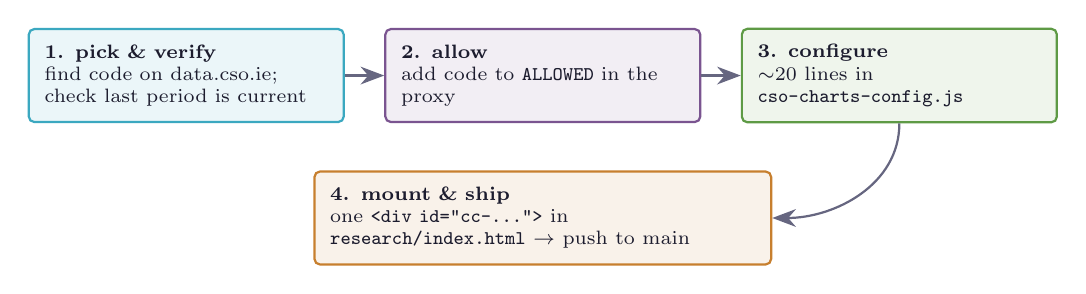
\begin{tikzpicture}[node distance=3mm and 5mm]
  \node[step=accent, text width=36mm] (a) {\textbf{1. pick \& verify}\\find code on data.cso.ie; check last period is current};
  \node[step=mpurple, text width=36mm, right=of a] (b) {\textbf{2. allow}\\add code to \texttt{ALLOWED} in the proxy};
  \node[step=mgreen, text width=36mm, right=of b] (c) {\textbf{3. configure}\\$\sim$20 lines in \texttt{cso-charts-config.js}};
  \node[step=myellow, text width=54mm, below=6mm of b] (d) {\textbf{4. mount \& ship}\\one \texttt{<div id="cc-...">} in \texttt{research/index.html} $\to$ push to main};
  \draw[flow=mutedg] (a) -- (b);
  \draw[flow=mutedg] (b) -- (c);
  \draw[flow=mutedg] (c.south) to[out=-90,in=0] (d.east);
\end{tikzpicture}
\end{center}

No drawing code, no fetch code, no DOM code --- the engine owns all of it.
Full prose reference: \texttt{docs/cso-data-pipeline.md}.

\end{document}
